\documentclass[12pt]{article}
\usepackage[utf8]{inputenc}
\usepackage{fullpage}
\usepackage{graphicx}
\usepackage{url}
\usepackage{amsmath}
\usepackage{amssymb}
\usepackage{caption}
\usepackage{subcaption}
\usepackage{color,soul}% just to highlight missing info


\title{Report 2:
Gaussian Process Regression on Parkinson's disease data}
\author{Abdurasul Bobonazarov, s267331, \\ICT for Health attended in A.Y. 2021/22}
\date{November 25th, 2021}

\begin{document}

\maketitle
\section{Introduction}
Patients affected by Parkinson’s disease cannot perfectly control their
muscles. In particular they show tremor, they walk with difficulties and,
in general, they have problems in starting a movement. Many of them
cannot speak correctly, since they cannot control the vocal chords and
the vocal tract. 

Levodopa is prescribed to patients, but the amount of treatment should be increased as the illness progresses and it should be provided at the right time during the day, to prevent the freezing phenomenon. It would be beneficial to measure total UPDRS ((Unified Parkinson’s Disease Rating Scale) many times during the day in order to adapt the treatment to the specific patient. This means that an automatic way to measure total UPDRS must be developed using simple techniques easily managed by the patient or his/her caregiver.

One possibility is to use patient voice recordings (that can be easily obtained several times during the day through a smartphone) to generate vocal features that can be then used to regress total UPDRS.

Gaussian Process Regression (GPR) was used on the public dataset at \cite{UCI} to estimate total UPDRS, and the results were compared to those obtained with linear regression, showing the superiority of GPR. 

\section{Data analysis}
The 22 features available in the dataset at \cite{UCI} are listed in table \ref{ta:feat}: of these, subject ID and test time were removed, total UPDRS is the regressand. All the remaining 19 features were used as regressors in linear regression, but only 3, namely motor UPDRS, age and PPE, were used in GPR.

\begin{table}
    \centering
    \begin{tabular}{||c|l||c|l||c|l|}
    \hline
        1 & subject & 2 & age & 3 & sex\\
        4 & test time & 5 & motor UPDRS & 6 & total UPDRS\\
        7 & Jitter(\%) & 8 & Jitter(Abs) & 9 & Jitter:RAP\\
        10 & Jitter:PPQ5 & 11 & Jitter:DDP & 12 & Shimmer\\
        13 & Shimmer(dB) & 14 & Shimmer:APQ3 & 15 & Shimmer:APQ5\\
        16 & Shimmer:APQ11 & 17 & Shimmer:DDA & 18 & NHR\\
        19 & HNR & 20 & RPDE & 21 & DFA\\
        22 & PPE &     &      &    &  \\
        \hline
    \end{tabular}
    \caption{List of features}
    \label{ta:feat}
\end{table}
The number of points in the dataset is 5875; data are shuffled and the first 50\% of the points are used to train the linear model, 25\% of the points are used for the validation and the remaining 25\% are used to test the model performance. Data are normalized using mean and standard deviation measured on the training dataset.

\section{Gaussian Process Regression}
In GPR, it is assumed that $N-1$ measured datapoints $(\mathbf{x}_k,y_k)$ are available in the training dataset, and that a new input  $\mathbf{x}_N$ is present, whose corresponding output $y_N$ has to be estimated. 

In the following, $\mathbf{Y}_L=[Y_1,\ldots,Y_L]$ is the $L$-dimensional random vector that includes the random variables $Y_\ell$ and $\mathbf{y}_{L}=[y_1,\ldots,y_{L}]$ is the $L$-dimensional vector that stores the measured values of $Y_\ell$. Vector $\mathbf{x}_\ell$ stores instead the measured regressors for $Y_\ell$. The random variable to be estimated is $Y_N$, knowing the corresponding regressors $\mathbf{x}_N$, and the training dataset made of $N-1$ measured couples $(\mathbf{x}_\ell,y_\ell)$, $\ell=1,\ldots,N-1$.
\begin{itemize}
\item The $N \times N$ covariance matrix $\mathbf{R}_{Y,N}$ of $\mathbf{Y}_N$ has $n,k$ value:
\[ \mathbf{R}_{Y,N}(n,k)=\theta \exp\left(-\frac{\|\mathbf{x}_n-\mathbf{x}_k\|^2}{2 r^2}\right)+\sigma_\nu^2\delta_{n,k},\quad n,k \in [1,N]\]
\item $\mathbf{R}_{Y,N}$ can be rewritten as
\[ \mathbf{R}_{Y,N}=
\begin{bmatrix}
\mathbf{R}_{Y,N-1} & \mathbf{k}\\
\mathbf{k}^T & d\\
\end{bmatrix}
\]
where $\mathbf{R}_{Y,N-1}$ is the covariance matrix of $\mathbf{y}_{N-1}$.
\item Then the pdf of $Y_N$ given the measured values $\mathbf{y}$ of $\mathbf{y}_{N-1}$ is
\[ f_{Y_N|\mathbf{y}_{N-1}=\mathbf{y}}(z)=\frac{1}{\sqrt{2\pi \sigma^2}}e^{-\frac{(z-\mu)^2}{2\sigma^2}}\]
\begin{equation} \mu=\mathbf{k}^T \mathbf{R}_{Y,N-1}^{-1}\mathbf{y}
\label{eq:mu}
\end{equation}
\begin{equation} \sigma^2=d-\mathbf{k}^T \mathbf{R}_{Y,N-1}^{-1}\mathbf{k}
\label{eq:sigma}
\end{equation}
The point estimation of $Y_N$ is $\hat{y}_N=\mu$.
\item In the above equations, couples $(\mathbf{x}_\ell,y_\ell)$ for $\ell=1,\ldots, N-1$ belong to the training dataset, couple $(\mathbf{x}_N,y_N)$ belongs to the test or to the validation dataset. 
\end{itemize}

The model hyperparameters are three: $\theta$, $r^2$ and $\sigma_\nu^2$. Since the training dataset stores normalized data, and $\sigma^2_\nu$ is small, parameter $\theta=\mathbf{R}_{Y,N}(n,n)$ (variance of $y_n$) was set equal to 1. 
Hyperparameters $r^2$ and $\sigma_\nu^2$ were set to minimize the mean square error $\mathbb{E}\{[y_N-\hat{y}_N]^2\}$ for the validation dataset. In particular, for each point $(\mathbf{x}_N,y_N)$ in the validation dataset, the $N=10$ closer points in the training dataset were found, a set of possible values for $r^2$ and $\sigma_\nu^2$ was tried and the optimum values were found among the considered cases (see Fig. \ref{fig:GPR_optim}): these optimum values are $r^2_{opt}=3.5$ and  $\sigma^2_{opt}=10^{-4}$.

Fig. \ref{fig:GPR_regr} shows $\hat{y}$ versus $y$ whereas Fig. \ref{fig:GPR_regr_err} also shows the error bars ($\pm 3\sigma_y$ where $\sigma_y$ is the denormalized version of $\sigma$ in \eqref{eq:sigma}). The estimation error histogram is shown in Fig. \ref{fig:GPR_hist}. Figs. \ref{fig:GPR_regr_err}-\ref{fig:GPR_hist} were obtained using   $r^2_{opt}$ and  $\sigma^2_{opt}$.
\begin{figure}
\centering
\begin{subfigure}{0.45\textwidth}
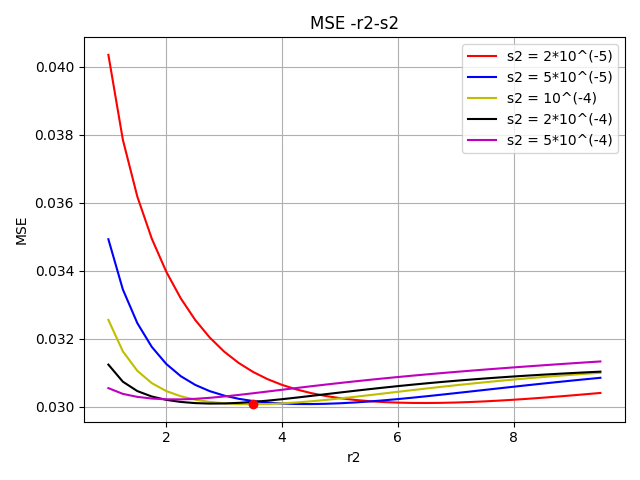
\includegraphics[width=\textwidth]{optimization.png}  
\caption{Optimization of \texttt{r2}=$r^2$ and \texttt{s2}=$\sigma_\nu^2$.}
\label{fig:GPR_optim}
\end{subfigure}
\begin{subfigure}{0.45\textwidth}
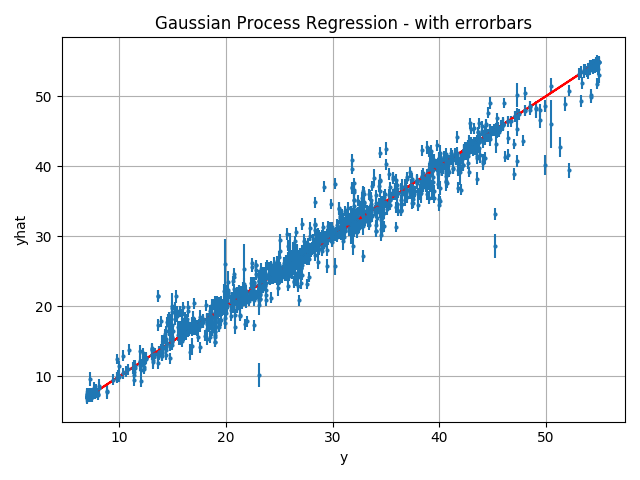
\includegraphics[width=\textwidth]{GP_regression_errorbars.png}  
\caption{$\hat{y}$ versus $y$ with errorbars for the test dataset.}
\label{fig:GPR_regr_err}
\end{subfigure}
\begin{subfigure}{0.45\textwidth}
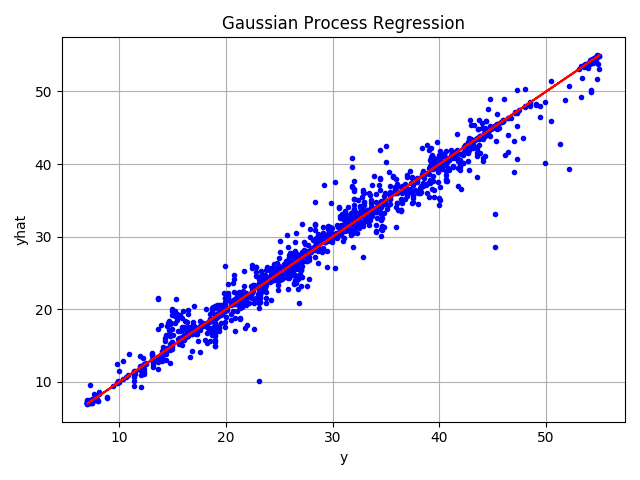
\includegraphics[width=\textwidth]{GP_regression.png}  
\caption{$\hat{y}$ versus $y$ for the test dataset.}
\label{fig:GPR_regr}
\end{subfigure}
\begin{subfigure}{0.45\textwidth}
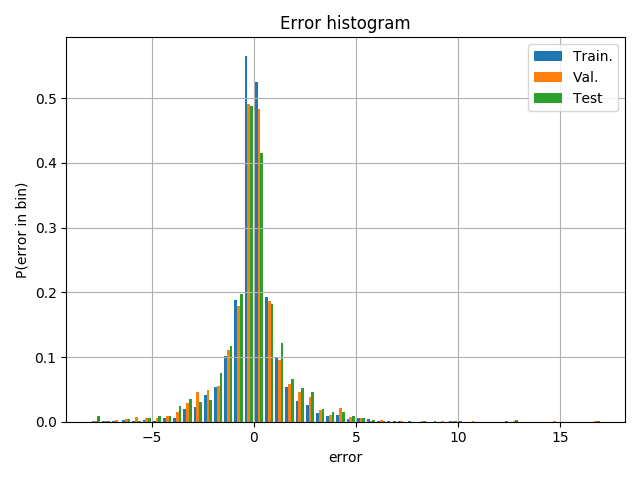
\includegraphics[width=\textwidth]{GP_error_hist.png} \caption{Histogram of $y-\hat{y}$ for training, validation and test datasets.}
\label{fig:GPR_hist}
\end{subfigure}
\caption{Gaussian Process Regression results.}
\label{fig:GPR}
\end{figure}


\section{Linear regression based on Linear Least Squares}
The model assumed in linear regression is
\begin{equation}
Y=w_1X_1+\ldots +w_{F}X_{F}=\mathbf{X}^T\mathbf{w}
\label{eq:lin_regr}
\end{equation}
where $Y$ is the regressand (total UPDRS), $\mathbf{X}^T=[X_1, \ldots, X_{F}]$ stores the $F$ regressors\footnote{$\mathbf{X}$ is a column vector and $\mathbf{X}^T$ is its transpose} and $\mathbf{w}^T=[w_1,\ldots,w_{F}]$ is the weight vector to be optimized. In (\ref{eq:lin_regr}), $Y, X_1, \ldots, X_{F}$ are all random variables.

Linear Least Squares (LLS) minimizes  the mean square error (MSE) and the optimum weight vector $\mathbf{w}$ can be obtained in closed form as:
\begin{equation}
\hat{\mathbf{w}}=\mbox{arg min }\mathbb{E}\{(Y-\mathbf{X}^T\mathbf{w})^2\}  =\left(\mathbf{\underline{X}}^T\mathbf{\underline{X}} \right)^{-1}\mathbf{\underline{X}}^T \mathbf{y}
\end{equation}
where $\mathbf{\underline{X}}$ is the matrix that stores the (normalized) training regressor points and $\mathbf{y}$ is the (normalized) training regressand vector.
Given $\hat{\mathbf{w}}$, the normalized regressand is estimated as
\begin{equation}
\hat{y}_N=\mathbf{x}_N^T\hat{\mathbf{w}}
\end{equation}

Figure \ref{fig:LLS} shows the results obtained with LLS. Note that, to get a meaningful comparison with GPR, the training dataset and test datasets with the two regression models are the same; the validation dataset was only used for GPR, not for LLS regression.

\begin{figure}
\centering
\begin{subfigure}{0.45\textwidth}
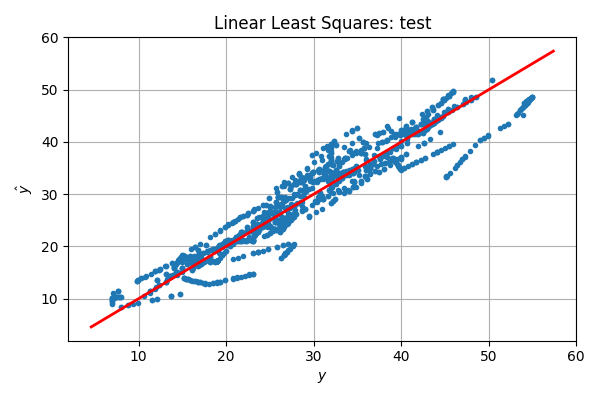
\includegraphics[width=\textwidth]{regression.png}  
\caption{$\hat{y}$ versus $y$ for test dataset.}
\label{fig:LLS_regr}
\end{subfigure}
\begin{subfigure}{0.45\textwidth}
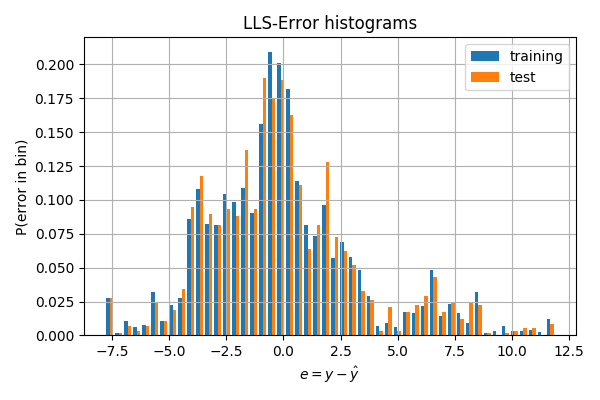
\includegraphics[width=\textwidth]{hist_err.png}    
\caption{Histogram of $y-\hat{y}$ for training, validation and test datasets.}
\label{fig:LLS_hist}
\end{subfigure}
\caption{Linear Least Squares results.}
\label{fig:LLS}
\end{figure}


\section{Comparison}

It is evident, by comparing Figs. \ref{fig:GPR_regr} and \ref{fig:LLS_regr} that, with the Parkinson's dataset, Gaussian Process Regression (GPR) is more precise than linear regression, and this is also confirmed by the estimation error histograms in Figs. \ref{fig:GPR_hist} and \ref{fig:LLS_hist}. 

Table \ref{ta:res} lists the main statistical properties of the estimation error $e=y-\hat{y}$ for the training and test datasets.
The mean square error of GPR is about 1/3 than that of LLS. 

\begin{table}[h]
    \centering
    \begin{tabular}{|l|l|c|c|c|c|}
    \hline
&  Dataset      & Err. Mean & Err. St. dev. & MSE & $R^2$\\
\hline
LLS &Training   & $-5.86*10^{-14}$  & 3.37  & 11.36  & 0.9881\\
    &Test       & $-2.65*10^{-2}$  & 3.31  & 10.95  & 0.9883\\
\hline
GPR &Training   & 0.0181  & 1.391  & 1.935  & 0.9971\\
    &Test       & 0.0061  & 1.829  & 3.345  & 0.995\\
\hline
    \end{tabular}
    \caption{Numerical comparison between GPR and LLS.}
    \label{ta:res}
\end{table}

\section{Conclusions}

Results show that the GPR consistently managed to outperform the LLS scores. For instance, Error Standard deviation of GPR is around twice lower than that of LLS. And, the coefficient of determination of GPR is also quite good (nearer to 1) comparing with that of LLS. Additionally, both methods do not show overfitting problem with the dataset.\\
It should be taken into account that these results are achieved using most relevant features (which are age, motor UPDRS and PPE) to predict total UPDRS. As the error standard deviation of GPR is much smaller than total UPDRS standard deviation value.\\
However, as the doctors have to measure the motor UPDRS and PPE in order to use regression methods, it does not have time saving advantage. So, it is not acceptable from medical point of view, as the total UPDRS cannot be measured without medical examination of a neurologist.


\begin{thebibliography}{9}
\bibitem{UCI} \url{https://archive.ics.uci.edu/ml/datasets/Parkinsons+Telemonitoring}

\end{thebibliography}
\end{document}
